\section{Cscope用法要略}

生成数据库:cscope -Rbq 
R表示递归,b表示build后不进入cscope自带的查询界面,q表示quick,加速日后的查询。

在vim下使用时应添加数据库,cs show命令显示当前已经添加的数据库,执行cs add cscope.out添加当前目录下cscope.out文件作为数据库。可以通过修改.vimrc来自动添加当前目录和父目录下的数据库。

\begin{verbatim}
"for cscope
if has("cscope")
        set csprg=/usr/bin/cscope
        set csto=0
        set cst 
        set nocsverb
        " add any database in current directory
        if filereadable("cscope.out")
                cs add cscope.out
        elseif filereadable("../cscope.out")
                cs add ../cscope.out
        elseif filereadable("../../cscope.out")
                cs add ../../cscope.out
                " else add database pointed to by environment
        elseif $CSCOPE_DB != ""
                cs add $CSCOPE_DB
        endif
        set csverb
endif

\end{verbatim}

在vim下键入:cs可以查看相关操作提示。具体用法参考见:h cscope或cscope的man页。

\begin{verbatim}
 USAGE   :cs find {querytype} {name}

            {querytype} corresponds to the actual cscope line
            interface numbers as well as default nvi commands:

                0 or s: Find this C symbol
                1 or g: Find this definition
                2 or d: Find functions called by this function
                3 or c: Find functions calling this function
                4 or t: Find this text string
                6 or e: Find this egrep pattern
                7 or f: Find this file
                8 or i: Find files #including this file

\end{verbatim}

可以在vim中添加一些键映射:

\begin{verbatim}
 nmap <F2>s :cs find s <C-R>=expand("<cword>")<CR><CR>
nmap <F2>g :cs find g <C-R>=expand("<cword>")<CR><CR>
nmap <F2>c :cs find c <C-R>=expand("<cword>")<CR><CR>
nmap <F2>t :cs find t <C-R>=expand("<cword>")<CR><CR>
nmap <F2>e :cs find e <C-R>=expand("<cword>")<CR><CR>
nmap <F2>f :cs find f <C-R>=expand("<cfile>")<CR><CR>
nmap <F2>i :cs find i ^<C-R>=expand("<cfile>")<CR>$<CR>
nmap <F2>d :cs find d <C-R>=expand("<cword>")<CR><CR>

nmap <F3>s :scs find s <C-R>=expand("<cword>")<CR><CR>
nmap <F3>g :scs find g <C-R>=expand("<cword>")<CR><CR>
nmap <F3>c :scs find c <C-R>=expand("<cword>")<CR><CR>
nmap <F3>t :scs find t <C-R>=expand("<cword>")<CR><CR>
nmap <F3>e :scs find e <C-R>=expand("<cword>")<CR><CR>
nmap <F3>f :scs find f <C-R>=expand("<cfile>")<CR><CR>
nmap <F3>i :scs find i ^<C-R>=expand("<cfile>")<CR>$<CR>
nmap <F3>d :scs find d <C-R>=expand("<cword>")<CR><CR>

\end{verbatim}









\section{Ctags关键用法}

创建元数据:
\begin{verbatim}
  ctags -R
\end{verbatim}
  对于C++,结合omnicppcomplete插件,有:
\begin{verbatim}
   ctags -R --c++-kinds=+p --fields=+iaS --extra=+q
\end{verbatim}

为vim配置tags搜索路径:
在.vimrc中添加设置。如使用绝对路径:
\begin{verbatim}
 set tags=/home/xxx/myproject/tags
\end{verbatim}

如果设置成自动搜索上级目录的tags:
\begin{verbatim}
set tags=./tags;
\end{verbatim}
注意第一行的分号表示递归向上搜索,点斜杠表示当前文件所在目录而非当前目录。

\begin{verbatim}
:set tags=./tags,./../tags,./*/tags
\end{verbatim}
使用当前目录下的tags文件, 上一级目录下
的tags文件, 以及当前目录下所有层级的子目录下的tags文件.


\begin{verbatim}
:set tags=~/proj/**/tags
\end{verbatim}
一种深度搜索目录的形式

查找:
\begin{verbatim}
vim -t tag名
:ta tag名
:tselect tag名 同名tag选择

\end{verbatim}

跳转:
\begin{verbatim}
Ctrl+]  跳转至函数定义
ctrl+O 返回
ctrl+I 前进
Ctrl+T 返回(与ctrl+])对应
:tp  同名tag,跳转到前一个
:tn  同名tag,跳转到下一个
:tfirst, :tlast 
\end{verbatim}


裂屏显示:
\begin{verbatim}
Ctrl-W ] 裂屏跳转至函数定义
[vertical] stag name 裂屏查找并跳转
\end{verbatim}



\section{数据文件分析工具}

\subsection{十六进制显示}

od, hexdump等工具将文件按照8进制、16进制、ASCII等形式打印出来。hexdiff同时打开两个文件,进行比较。

\subsection{十六进制编辑}
hexer工具能够以vi风格的界面编辑数据文件,而ghex则基于Gnome窗口系统。其他工具大多基于curses家族,包括hexedit, lfhex, dhex等。

\subsection{其他}

strings:寻找文件中的字符串。可用于分析可执行文件。
\section{Doxygen文档生成工具}
\begin{verbatim}
http://www.stack.nl/~dimitri/doxygen/index.html

http://sourceforge.net/projects/doxygen/
\end{verbatim}

\begin{shellcmd}
doxygen -g
doxygen Doxyfile
\end{shellcmd}

要点:
\begin{enumerate}
	\item 修改Doxyfile,可以指定项目名称,概要,语言(Chinese)等。Doxyfile中比较重要的字段还包括
	\begin{enumerate}
		\item OUTPUT\_LANGUAGE
		\item OPTIMIZE\_OUTPUT\_FOR\_C
		\item EXTRACT\_ALL, EXTRACT\_STATIC
	\end{enumerate}
	\item \verb+ \mainpage \author +等命令比较常用
	\item 无需学习过多内容
\end{enumerate}

在vim中安装doxygen-toolkit插件,常用命令包括
\begin{verbatim}
:Dox
生成函数注释
\end{verbatim}

\section{GDB调试器使用要略}


如果想对elfname程序进行调试,则:
\verb+gdb elfname+或\verb+gdb --args elfname arg1 arg2+\ldots
也可以只输入gdb,在交互界面上设置:
file elfname;
set args argv1 argv2 \ldots 

该程序在编译时需使用-g选项。

基本的用法,可以在进入gdb后执行help。

每次执行run,会从头开始运行程序。run简称r。

\subsection{查看源码}
list 显示当前位置10行代码。list简称l。

list funcname:显示某函数附近的10行代码

list lineno: 显示第lineno行及其上下文10行代码


\subsection{断点}
help b可以查看断电的用法。

首先需要明确,如果在第18行设置断点,指的是在第18行执行之前中止,而非之后。

设置断点:breakpoint命令,简称b,参数为[文件名:]行号或函数名,可以用list命令辅助b命令的参数选择。如无参数,为在当前行设置断点。

此外,断点还可以enable, delete, disable。

delete b会删除所有断点。简称del b或del或d。del 2会删除2号断点。

info breakpoints,简称info b,显示当前断点。

遇到断点时执行cont或c时程序继续执行直至结束或受阻。

commands 断点号:
用于修改断点行为。如 
\begin{verbatim}
commands 2
>display
>end
\end{verbatim}
程序在2号断点不中止,而是执行display;end用于退出对commands的定义。

\subsection{步进}
next命令简称n,用于执行下一条语句。执行完后显示的代码行为尚未执行的下一条语句。

n 5可以前进5行。

Return键用于重复执行上一条命令。

step命令简称s,与next的区别是会进入函数体。

\subsection{查看上下文信息}

backtrace, 简称bt,查看堆栈层次信息。最内层的frame号为零;

命令 frame frameno会跳到frameno指定的frame层次并打印相关信息。

在函数堆栈中,info args为函数参数;在main函数中则为程序参数。

info line 显示当前行号。

info source 查看当前源文件信息。info sources查看所有源文件信息。

info locals 局部变量信息查看。

info variables 查看全局变量和静态变量。

info registers,info frame顾名思义。

info macro macroname和info macros查看宏定义。


\subsection{查看指定变量}
print varname 查看变量。print简称p。

例如,对于char c[5] = {97,98,99,100,101},
执行print c[2]显示 99 'c';print /x c[2]会显示为16进制0x63。
print /x c[2]@3会显示c[2]开始的3个连续变量{0x63, 0x64, 0x65}。

display varname 添加自动显示变量。
display添加的变量会在每次程序中止时再次显示。

\subsection{Patching:就地修补}
set variable varname = varvalue命令用于就地修改变量的值。
那么,下面的命令在断点处修改变量的值,下次run时生效。
\begin{verbatim}
commands 2
>set variable n = n+1
>cont
>end
\end{verbatim}


\subsection{观察值}
watch varname命令:当程序执行时发现varname被修改时就中止;
rwatch varname:当varname被读时中止;而awatch是在varname被读或者写时都中止。

注意watch只能观察当前堆栈frame的变量。所以一般要配合断点来使用。









































\section{git用法}

\begin{figure}[htpb]
    \begin{center}
        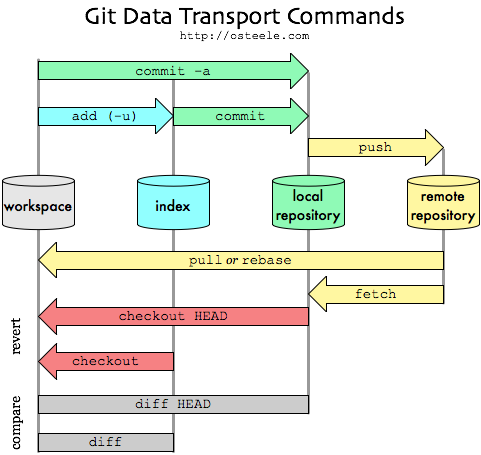
\includegraphics[keepaspectratio,width=0.5\paperwidth]{Pictures/git_dataflow.png}
    \end{center}
    \caption{Git数据流}
\end{figure}

\subsection{配置}
配置彩色界面
\begin{verbatim}
git config --global color.ui true
\end{verbatim}

\subsection{基本用法}
创建版本库

\begin{verbatim}
git init
\end{verbatim}

添加文件并提交

\begin{verbatim}
git add -A
git commit -m ``initialized''
\end{verbatim}


修改文件并提交
\begin{verbatim}
git commit -a
\end{verbatim}

撤销工作区修改
\begin{verbatim}
git checkout -- . 撤销修改,用暂存区覆盖工作区
git checkout .  同上
\end{verbatim}

查看历史
\begin{verbatim}
git log <refs>本分支提交历史
git log -3 只显示最近3次提交
git log --stat 显示修改统计
git reflog [show] <refs> 引用历史
\end{verbatim}

查看文件状态
\begin{verbatim}
git checkout [HEAD] 显示工作区、暂存区、HEAD之间的差异
git status
git ls-files [-c] 查看暂存区文件
git ls-files -m 查看被修改的文件
git ls-files -d 查看被删除的文件
git ls-files -o 查看其他文件,即未被追踪的文件
git write tree; git ls-tree <treeish> 查看tree包含的blob
\end{verbatim}

检出历史文件
\begin{verbatim}
git checkout <commit> [--] filename
省略commit,则表示暂存区。
\end{verbatim}

整体回归历史
\begin{verbatim}
git reset --hard <id> 
提交日志也会一起回归历史
git checkout <id> 
会进入分离头指针状态,此后的提交日志不容易查看
git checkout -b <new_branch> <id>
新建分支,回归历史
\end{verbatim}
总之,checkout命令修改HEAD指向,reset修改分支指向

修改刚才的提交的提交说明
\begin{verbatim}
git commit --amend
\end{verbatim}

修改某个历史提交的提交说明
\begin{verbatim}
git rebase -i <some history>
\end{verbatim}

将从v1开始的历次提交逐一导出为补丁
\begin{verbatim}
git format-patch v1..HEAD
\end{verbatim}

不慎提交了不想提交的文件,如winxp.img
\begin{verbatim}
git rm --cached winxp.img
git commit --amend
\end{verbatim}
git rm将文件从工作区和index同时删除。--cache指定不从工作区删除。

比较差异:
比较工作区和暂存区:git diff
比较工作区与HEAD:git diff HEAD
比较工作区与里程碑A:git diff A
比较暂存区与里程碑A:git diff --cached A
比较暂存区与HEAD:git diff --cached
比较里程碑A和B git diff B A

\subsection{显示id}
\begin{verbatim}
git rev-parse master
\end{verbatim}

创建里程碑``v1''
\begin{verbatim}
git tag v1
\end{verbatim}




\section{Indent代码排版工具}

欲实现Cavium风格的代码,有
\begin{verbatim}
indent *.c -bli0 -i4 -npsl -cli4 -npcs
\end{verbatim}

其中,bli表示brace indentation, i选项表示indentation, npsl(dont-break-procedure-type)表示函数返回类型需与函数名称在同一行;cli表示case-label-indentation, 表示case语言缩进的距离。npcs表示no-sapce-after-function-call-names,函数调用时函数名称后无空格。

关于if等语句之后的\verb+{+括号是否在换行,有两种方式:br(braces-on-if-line)和bl(braces-after-if-line)。对于br选项,一般同时指定ce选项(cuddle-else)或nce选项,前者让\verb+}+和else在同一行。对于bl选项,一般同时指定bli选项,表示\verb+{+缩进距离,如不指定,GNU indent默认使用GNU风格,即缩进2个空格。类似于if语句,函数定义和struct定义也存在大括号是否在同一行的问题。对于函数,可以指定brf或blf(默认);对于struct,可以指定brs和blf。
\section{Nerd注释插件用法}
\begin{verbatim}
简单介绍下NERD Commenter的常用键绑定,以C/C++文件为例,详析的使用方法,请:h NERDCommenter。在Normal或者Visual 模式下:

,ca,在可选的注释方式之间切换,比如C/C++ 的块注释/* */和行注释//

,cc,注释当前行

,c,切换注释/非注释状态

,cs,以”性感”的方式注释

,cA,在当前行尾添加注释符,并进入Insert模式

,cu,取消注释

Normal模式下,几乎所有命令前面都可以指定行数

Visual模式下执行命令,会对选中的特定区块进行注释/反注释

注:各命令前缀是可以自己设置的,通常是逗号’,'或者’\’.
\end{verbatim}
\section{Python IDE选用}

\subsection{Vim搭建Python IDE}
Vim插件pythonComplete可用于Python代码自动补全。对于VIM 7.3以上版本,这个插件是自带的。需要在.vimrc上添加如下配置:
\begin{verbatim}
filetype plugin on  
autocmd FileType python set omnifunc=pythoncomplete#Complete  
\end{verbatim}

\subsection{ctags配置}
ctags也支持Python语言:
\begin{verbatim}
ctags -R
ctags -R --language-force=Python --Python-kinds=cfmvi --extra=+q
\end{verbatim}

\subsection{Eric}
Eric是基于Qt的IDE,依赖于包python-qscintilla2。

\subsection{IDLE}
IDLE常常是python安装是自带的开发工具。

\section{Subversion版本修订控制}
checkout(co)操作

\begin{verbatim}
svn checkout http://svn.example.com:9834/repos
svn checkout file:///var/svn/repos
svn co https://svn.sinaapp.com/myhello(新浪云平台) 
\end{verbatim}

添加文件:
\begin{verbatim}
svn add DIRNAME/
\end{verbatim}

提交文件:
\begin{verbatim}
svn ci -m ``MESSAGE''
\end{verbatim}






\section{Vim之taglist插件}
用法:
\begin{verbatim}
:TlistToggle 打开或关闭列表
<CR> 跳转至列表所指对象
<Space> 显示原型
u 更新列表
s 更新排序方式(按出场顺序或名称)
x 伸缩列表宽度
\end{verbatim}

常见设置(.vimrc)
\begin{verbatim}
let Tlist_Show_One_File = 1            "不同时显示多个文件的tag,只显示当前文件的
let Tlist_Exit_OnlyWindow = 1          "如果taglist窗口是最后一个窗口,则退出vim
let Tlist_Use_Right_Window = 1         "在右侧窗口中显示taglist窗口
let Tlist_GainFocus_On_ToggleOpen = 1
map <silent> <leader>tl :TlistToggle<cr>
\end{verbatim}


\section{UML正反向工程}
umbrello:不能包含c语言标准库的文件,如
\verb+#include <time.h>+
否则程序会崩溃
\section{Vim文本编辑}


\subsection{快速键入}
本节C表示Ctrl键。
在insert模式下:\\
C-W 删除当前单词(同Bash) \\
C-U 删除当前句子(同Bash)\\
C-P,C-N  自动补全,补全内容分别从前方或后方搜索\\
C-A 键入上次在INSERT模式下键入的内容,并进入INSERT模式\\
C-Y 键入上次在INSERT模式下键入的内容\\
C-X C-F 自动补全,文件名\\
C-X C-L 自动补全,整行\\
C-X C-D  自动补全,宏定义\\

在Normal模式下,CTRL A 和CTRL X分别将光标下的数字加1或减1

\subsection{快速配对区域操作}
快速处理\verb+''、""、()、[]、{}、<> +等配对标点符号中的文本内容,包括更改、删除、复制等。
\begin{verbatim}
ci(  快速修改()内的内容,即删除后进入insert模式
di(  快速删除()内的内容
yi(  快速复制()内的内容
\end{verbatim}
将上述i替换为a,()本身也会被选取。


\subsection{跨文档复制粘贴}
一般地,复制到指定寄存器的方法为:

普通模式下\verb|"+寄存器名+y|。

插入某寄存器内容的方法为:

普通模式下\verb|"+寄存器名+p|或编辑模式下\verb|Ctrl+R+寄存器名|。

有两个特殊的寄存器: 选择寄存器(寄存器``)为可视模式下选择的内容,剪贴板(寄存器+)为用图形界面选择的内容。


\subsection{跨文件字符替换}
每个文件在vim被称为缓冲区。

方法一:命令录制。
\begin{verbatim}
qq,:wnext,q.
\end{verbatim}

方法二:bufdo, argdo, windo等。
\begin{verbatim}
:wa
:bufdo %s/foo/bar/ge |update
\end{verbatim}

\subsection{文档统计}
显示当前文件名称与行数
\begin{verbatim}
:f 或 Ctrl+G
\end{verbatim}
显示某单词word出现的次数
\begin{verbatim}
%s/word//gn
\end{verbatim}
中文字数统计(近似方法)
\begin{verbatim}
%s/\S//gn
缺点是将非中文字符也算做一个字,如英文单词、标点等。
:%s/[^[:print:][:cntrl:]]//gn
缺点是中文标点也算作了汉字
:%s/[\u4e00-\u9fa5]//gn
使用unicode匹配,不成功,可能是因为utf8编码的文件不支持unicode匹配
\end{verbatim}


注意wc -m命令也可以统计字符数,但是把空白字符也算作内了。

\subsection{基于空格的列操作}
\verb+\S,\s+分别表示非空格和空格,后带\verb%\+%表示至少为一。再结合括号和数字引用,可以基于空格进行各种列操作。

例1:在非空行前后添加内容:
\verb#:%s/^\s*\(\S\+.*\)$/haha;\1wawa;#

例2:只保留第一列,其余删除:
\verb%5,12s/\(\S\+\)\s\+.*/\1/g%

\subsection{折行的开与关}
zR 打开所有折行;zr打开下一级折行;zM关闭所有折行;zm 关闭上一级折行
zo 打开折行;zc 重新关闭折行
zf 创建折行;zfap zf命令作用于ap(一个段落)

\subsection{屏幕错乱}
Ctrl+L即可。

\subsection{键入特殊字符}
外国人姓名之间的点号:fcitx激活时键入[即可。
\begin{verbatim}
:digraphs 查看VIM支持的特殊字符
\end{verbatim}
Insert模式使用CTRL-K {key1 key2}键入特殊字符。
如输入拼音a的四个声调,分别为\verb+a-(或a~),a‘,a<,a`(或a!)+。希腊字符\[\alpha,\beta\]分别为\verb+a*, b*+。

\subsection{键入Unicode字符}
Insert模式使用CTRL-V {digits}来插入一个由{digits}指定其ASCII码的字符. 

用这种方法你可以插入0到255的所有字符.如果你键入的数字少于两个, 那么Vim会在遇到一个非数字字符时终止这个命令. 要避免非得键入一个非数字字符才能让这个命令结束,你可以在数字前加上一个或两个0来凑足3个数.

\begin{verbatim}
CTRL-V 009.
\end{verbatim}

要用十六进制来表示你的ASCII, 在CTRL-V后面附加一个"x":
\begin{verbatim}
CTRL-V x7f
\end{verbatim}

接下来的两个方法还可以让你键入一个16bit或32bit的数字(比如,用来指定一个Unicode字符):
\begin{verbatim}
CTRL-V o123
CTRL-V u1234
CTRL-V U12345678
\end{verbatim}

\subsection{快速插入日期}
可以定义如下键盘映射,使得在Insert模式下,F8可以键入日期:
\begin{verbatim}
imap <F8> <Esc>:read !date +\%F<CR>i
使用了date系统命令,\是为了转义%号,在Bash中不需要
格式%F相当于%Y-%m-%d
\end{verbatim}

\subsection{大小写替换}
在替换命令中,一个字符前面加\verb+\u+会被转为大写,\verb+\l+会被转为小写。


\subsection{列选择模式}
Normal模式下CtrlV会进入列选择模式,可以用来对表格的列进行选择操作。


\subsection{缩写}
iab命令定义在Insert模式下的缩写,如

\begin{verbatim}
iab ssend SSEND_HAHA
\end{verbatim}
iunab取消缩写,iab列出缩写。

\subsection{C程序缩进}
设置缩进为4,并用空格代替TAB:
\begin{verbatim}
set softtabstop=4
set shiftwidth=4
set expandtab
\end{verbatim}
== 为当前行整理缩进
=a{ 为当前代码块整理缩进
=G 从当前行到文件结尾,整理缩进
gg=G 为整个文件整理缩进


\subsection{英文拼写检查}
\begin{verbatim}
:setlocal spell spelllang=en_us 
:set spell
:setlocal nospell
:set nospell
\end{verbatim}


\subsection{vim选项的值}
\begin{verbatim}
:se[t] 显示所有不等于默认值的选项
:set all 显示所有选项
:set option? 显示选项的值
:set option 对于Toggle类型的选项,将其值设置为on;其他类型的选项,显示其值
\end{verbatim}

\subsection{重新载入vimrc}
\begin{verbatim}
:source ~/.vimrc
:so ~/.vimrc
\end{verbatim}


\section{在Vim中编写tex文件}

\subsection{latexsuite安装与配置}
\begin{shellcmd}
	sudo apt-get install vim-latexsuite
	vim-addons install latex-suite
\end{shellcmd}
意欲在打开tex文件时自动开启latexsuite,需配置.vimrc
详细参见help:latex-suite
\begin{verbatim}
    " REQUIRED. This makes vim invoke Latex-Suite when you open a tex file.
    filetype plugin on
    
    " IMPORTANT: win32 users will need to have 'shellslash' set so that latex
    " can be called correctly.
    set shellslash
    
    " IMPORTANT: grep will sometimes skip displaying the file name if you
    " search in a singe file. This will confuse Latex-Suite. Set your grep
    " program to always generate a file-name.
    set grepprg=grep\ -nH\ $*
    
    " OPTIONAL: This enables automatic indentation as you type.
    filetype indent on
    
    " OPTIONAL: Starting with Vim 7, the filetype of empty .tex files defaults to
    " 'plaintex' instead of 'tex', which results in vim-latex not being loaded.
    " The following changes the default filetype back to 'tex':
    let g:tex_flavor='latex'

\end{verbatim}

\subsection{配置文件}
配置文件texrc的路径为:
~/.vim/ftplugin/latex-suite
\subsection{环境插入}
F5用于输入环境。

\subsection{分节}
文档上给出了快捷键:
\begin{verbatim}
SPA for part
SCH for chapter
SSE for section
SSS for subsection
SS2 for subsubsection
SPG for paragraph
SSP for subparagraph
\end{verbatim}


\subsection{借助sort命令多域排序}
如果以\&为分隔符(常见于latex表格),第二列升序,第一列降序排序,则有:
\verb+sort -k 2n -k 1r -t'&' FILENAME+

\subsection{表格标记添加}
如果表格是从word或网页上拷贝的,则需要添加\&和换行符号。在vim中依次执行一下命令:
\begin{verbatim}
:22,40s/\s\+$//  #去除行尾空格
:22,40s/\(\s\+\)/\&\1/g #空格前添加&
:22,40s/$/\\\\/g #行尾添加\\符号
\end{verbatim}



\section{Vim跳转}

\subsection{同时打开两个文件}
\begin{verbatim}
vim -o a.txt b.txt 竖屏
vim -O a.txt b.txt 横屏
vim -p a.txt b.txt 多标签页
:new 新增空白窗口
Ctrl-w = 平分宽高,注意键入=时,ctrl和w必须松开
Ctrl-w +/> 增减高/宽
Ctrl-w -/< 减小高/宽
Ctrl-w 20< 宽度减小20个单位
20Ctrl-w < 宽度减小20个单位
:vertical res[ize] +8 宽度增减8
\end{verbatim}

\subsection{命令行窗口}
Normal模式下键入\verb+q:+。

\subsection{shell跳转}
\begin{verbatim}
:sh 暂时返回shell;exit会返回vim
ctrl+Z 将vi转入后台,用fg恢复vi
\end{verbatim}

\subsection{路径跳转}
\begin{verbatim}
:E[xplore] 裂屏显示文件目录
:Sex 同Explore, 但是是上下裂屏
\end{verbatim}

\subsection{文件跳转}
\begin{verbatim}
:find filename用于文件跳转。
:[vert] sfind filename裂屏跳转。
:tabfind filename 新建标签页并跳转
gf(goto file)跳转到光标下的文件。
\end{verbatim}

有时需要添加path信息,如
\begin{verbatim}
:set path+=<path to the file>
:set path 显示path的当前值
:checkpath 显示所有无法找到的#include文件
:checkpath! 显示所有#include文件
\end{verbatim}
当前目录下的文件不需要添加path信息。

我们还可以在这个命令中使用通配符来进行匹配,如:
\begin{verbatim}
:set path=/usr/include,/usr/include/*
\end{verbatim}
这样,\verb+:find stdio.h+就可以查看一些库文件。

**匹配整个目录树,如:
\begin{verbatim}
:set path=/usr/include/**
:set path=/home/oualline/progs/**/include
\end{verbatim}
空字符串指当前目录,.指我们正在编辑的文件所在的目录,例如下面的命令是告诉Vim查找的目录包括/usr/include及其所的子目录,我们正编辑的文件所在的目录(.)以及当前目录(空串):
\begin{verbatim}
:set path=/usr/include/**,.,,
\end{verbatim}

\subsection{语句跳转}
\begin{verbatim}
[/]{ 查找上/下一个层次高于当前位置的{,用于语句块跳转
[/]# 查找上/下一个层次高于当前位置的#,用于在#ifdef-#endif结构中跳转
[/]( 查找上/下一个层次高于当前位置的(,用于在条件表达式中跳转
[/]/ 查找上/下一个层次高于当前位置的/,用于在注释中跳转
[/][ 查找上/下一个层次为1的{,用于全局函数跳转
[/]m 查找上/下一个层次为1或2的{,在面向对象语言中method对应层次为2的{
{/} 转到上/下一个空行
*/# 转到当前光标所指的单词下/上一次出现的地方
\end{verbatim}
[I 会列出所有包含该标识符的行,其中第一行可能包含变量定义,搜索范围包括了include文件。

[I命令查找任何的标识符.要只查找宏使用[D。

[d显示[D的第一个结果,[i显示[I的第一个结果。

[+tab 跳转至函数声明或变量定义,估计就是[i所指示的结果。gD将搜索范围局限在了当前文件,gd将搜索范围局限在了当前函数。

\subsection{标签页操作}

\begin{verbatim}
vim -p file1 file2 ..
:tabnew file1
:tabe[dit] file2
:tabnew
:tab split
:tabs 显示所有标签页的信息
\end{verbatim}
使用标签页打开文件

\begin{verbatim}
:tabc :q 关闭当前标签页
:tabo 关闭所有标签页
gt 转入下一个标签页
gT 转入上一个标签页
3gt 转入第3个标签页
:tabn 转入下一个标签页
:tabp 转入上一个标签页
:tabfirst, :tablast 顾名思义
:tabdo cmd 对所有标签页执行命令
\end{verbatim}





\section{Nerd注释插件用法}
\begin{verbatim}
简单介绍下NERD Commenter的常用键绑定,以C/C++文件为例,详析的使用方法,请:h NERDCommenter。在Normal或者Visual 模式下:

,ca,在可选的注释方式之间切换,比如C/C++ 的块注释/* */和行注释//

,cc,注释当前行

,c,切换注释/非注释状态

,cs,以”性感”的方式注释

,cA,在当前行尾添加注释符,并进入Insert模式

,cu,取消注释

Normal模式下,几乎所有命令前面都可以指定行数

Visual模式下执行命令,会对选中的特定区块进行注释/反注释

注:各命令前缀是可以自己设置的,通常是逗号’,'或者’\’.
\end{verbatim}
\section{Python IDE选用}

\subsection{Vim搭建Python IDE}
Vim插件pythonComplete可用于Python代码自动补全。对于VIM 7.3以上版本,这个插件是自带的。需要在.vimrc上添加如下配置:
\begin{verbatim}
filetype plugin on  
autocmd FileType python set omnifunc=pythoncomplete#Complete  
\end{verbatim}

\subsection{ctags配置}
ctags也支持Python语言:
\begin{verbatim}
ctags -R
ctags -R --language-force=Python --Python-kinds=cfmvi --extra=+q
\end{verbatim}

\subsection{Eric}
Eric是基于Qt的IDE,依赖于包python-qscintilla2。

\subsection{IDLE}
IDLE常常是python安装是自带的开发工具。

\section{Vim之quickfix插件}
Vim标准插件,无需安装。

在代码窗口中执行:make命令后,按回车可以定位到第一个error或warning。

用法:
\begin{verbatim}
:cc                显示详细错误信息 ( :help :cc )
:cp                跳到上一个错误 ( :help :cp )
:cn                跳到下一个错误 ( :help :cn )
:cl                列出所有错误 ( :help :cl )
:cw                如果有错误列表,则打开quickfix窗口 ( :help :cw )
:col               到前一个旧的错误列表 ( :help :col )
:cnew              到后一个较新的错误列表 ( :help :cnew ) 
\end{verbatim}

常见设置(.vimrc)
\begin{verbatim}
"quickfix
nmap <F6> :cn<cr>
nmap <F7> :cp<cr>
\end{verbatim}


\section{Vim之taglist插件}
用法:
\begin{verbatim}
:TlistToggle 打开或关闭列表
<CR> 跳转至列表所指对象
<Space> 显示原型
u 更新列表
s 更新排序方式(按出场顺序或名称)
x 伸缩列表宽度
\end{verbatim}

常见设置(.vimrc)
\begin{verbatim}
let Tlist_Show_One_File = 1            "不同时显示多个文件的tag,只显示当前文件的
let Tlist_Exit_OnlyWindow = 1          "如果taglist窗口是最后一个窗口,则退出vim
let Tlist_Use_Right_Window = 1         "在右侧窗口中显示taglist窗口
let Tlist_GainFocus_On_ToggleOpen = 1
map <silent> <leader>tl :TlistToggle<cr>
\end{verbatim}


